    \documentclass[12pt]{article}
    \usepackage[utf8]{inputenc}
    \usepackage{lmodern}
    \usepackage[T1]{fontenc}
    \usepackage{amsmath}
    \usepackage{enumitem}
    \usepackage{graphicx}
    \usepackage{fullpage}
    \usepackage{siunitx}
    \usepackage{fancyhdr}
    \PassOptionsToPackage{hyphens}{url}
    \usepackage[hyphens]{url}
    \usepackage{color}
    \usepackage{enumitem}
    \usepackage{textcomp}
    \usepackage{geometry}
    \usepackage{courier}
    \usepackage{listings}
    \usepackage{array}
    \usepackage{amsthm}
    \usepackage{mathdots}
    \usepackage{amssymb}
    \usepackage{minted}
    \usepackage{wrapfig}
    \usepackage{titlesec}
    \usepackage{parskip}
    \usepackage{accents}
    \usepackage{gensymb}
    \usepackage{indentfirst}
    \usepackage{courier}
    \usepackage{framed}
    \usepackage{etoolbox}
    \usepackage{titlesec}
    \usepackage{appendix}
    \usepackage{mdframed}
    \usepackage{verbatim}
    \usepackage{xspace}
    \usepackage{hyperref}
    \AtBeginEnvironment{subappendices}{%
        \section*{Appendix}
        \addcontentsline{toc}{section}{Appendices}
    }
    
    %\lstset{language=C++,
    %                basicstyle=\ttfamily,
    %                keywordstyle=\color{blue}\ttfamily,
    %                stringstyle=\color{red}\ttfamily,
    %                commentstyle=\color{green}\ttfamily,
    %                morecomment=[l][\color{magenta}]{\#}
    %}
    
    \definecolor{keywordcolor}{rgb}{0,0,0.45}
    \definecolor{stringcolor}{rgb}{0.45,0.45,0.45}
    \definecolor{commentcolor}{rgb}{0,0.3,0}
    
    \lstset{
        language=C++,
        basicstyle=\footnotesize\ttfamily,
        numbers=left,
        %numberstyle=\tiny,
        frame=tb,
        columns=fullflexible,
        showstringspaces=false,
        breaklines=true,
        tabsize=4,
        keywordstyle=\color{keywordcolor}\footnotesize\bf\ttfamily,
        stringstyle=\color{stringcolor}\footnotesize\ttfamily,
        commentstyle=\color{commentcolor}\it\sffamily
    }
    % \lstset{basicstyle=\ttfamily,breaklines=true}
    \lstloadlanguages{C++}
    
    %\renewcommand{\familydefault}{\sfdefault}
    
    \addtolength{\parskip}{\baselineskip}  
    \newcommand{\urlwofont}[1]{\urlstyle{same}\url{#1}}
    
    \renewcommand{\arraystretch}{0.8}
    \renewcommand{\headrulewidth}{0pt}
    \renewcommand{\footrulewidth}{0pt}
    
    \newcommand{\imagewidth}{0.8\textwidth}
    
    \lhead{}
    \chead{}
    \rhead{}
    \lfoot{}
    \cfoot{\thepage}
    \rfoot{}
    
    \geometry{
        top=0.9in,
        inner=0.7in,
        outer=0.7in,
        bottom=0.9in,
        headheight=2ex,
        headsep=1ex,
    }
    \pagestyle{fancy}
    %\fancyhf{}
    %\setlength{\headsep}{0.2in}
    
    
    \fancypagestyle{firststyle}
    {
        \chead{}
        \setlength{\headsep}{0.0in}
    }
    \hypersetup{
        unicode=true,
        colorlinks=true,
        linkcolor=blue,
        citecolor=black,
        filecolor=black,
        urlcolor=blue
    }
    
    \begingroup
    \makeatletter
    \@for\theoremstyle:=definition,remark,plain\do{%
        \expandafter\g@addto@macro\csname th@\theoremstyle\endcsname{%
            \addtolength\thm@preskip\parskip
        }%
    }
    \endgroup
    
    \newtheorem{thm}{Theorem}[section]
    \newtheorem{lemma}{Lemma}[section]
    \newtheorem{claim}{Claim}[section]
    \newtheorem{proposition}{Proposition}[section]
    %\theoremstyle{empty}
    \newtheorem*{namedthm}{Theorem}
    
    % indention size
    %\setlength{\parindent}{19pt}
    \setlength{\parindent}{0pt}
    
    % paragraph spacing
    \setlength{\parskip}{1em}
    
    % line spacing
    \linespread{1}
    
    %\setcounter{tocdepth}{1}
    
    
    % Documenting starts here! Please do not change above! 
    
    \newcommand{\mytitle}
    {
        \textbf {
            inzva Algorithm Programme 2018-2019\\ \ \\
            Bundle 14 \\ \ \\ 
            Algorithms - 5\\ \ \\
        }
    }
    
    \title{\vspace{-2em}\mytitle\vspace{-0.3em}}
    
    \author{
        \textbf{Editor}\\
        Mehmet Altuner  \\ \ \\ 
        \textbf{Reviewer} \\ Osman Karaketir
    }
    
    \date{}
    \begin{document}
        
        \begin{figure}
            \centering
            
\includegraphics[width=\linewidth/4]{inzva-logo.png}
            \label{fig:inzva}
        \end{figure}
        \maketitle
        
        \cleardoublepage
        \tableofcontents
        \markboth{Table of Contents}{}
        \cleardoublepage
        
        \section{Hashing}
        We can find a unique integer representation for each string. This process is called Hashing. There are a lot of hashing functions, we look into one of them: Polynomial rolling hash. \\
        
        Hash of string s with length k + 1 is: $hash(s) = (s[0] * p^{(k)}+ s[1] * p ^ {(k-1)} + ... + s[k] * p^0) \pmod{b}$ \\
    
        Choose $p$ as a prime number that is bigger than the size of the alphabet, choose $m$ as a large prime number to ensure that the hash value of the string is unique for that particular string.
        
        Popular $p$ and $m$ values are $p = 31$ and $m = 1e9 + 7$.
        
        \begin{minted}[frame=lines,linenos,fontsize=\footnotesize]{c++}
long long int hash_func(string text){
    int p = 271; // 
    long long int result_hash = 0;
    /*
    a prime number that is bigger than the size of 
    the alphabet. Alphabet size for char is 256.
    */
    long long int m = 1e9 + 7; // a very large number
    
    long long int p_pow = 1;
    
    for(int i= text.size() - 1; i>=0; i--){
        result_hash += (s[i]*p_pow) %m;
        result_hash = result_hash %m
        p_pow = p * p_pow;
    }

    return result_hash;
}
        \end{minted}
        
         We will make use Polynomial rolling hash in Rabin-Karp Algorithm for pattern finding.
        \newpage
        \section{String Matching Algorithms}
        
        \subsection{Basics}
        
        In string matching, our goal is to find a pattern in a given text. Sometimes we are asked only to find out if there is at least one matching substring or how many matching substring there are.
        
        \subsection{Naive Approach}
        In naive approach, we simply traverse through all possible substrings of length \texttt{m} of the given text of length \texttt{n}. We check each substring for whether it is matching with the given pattern or not. Therefore, our complexity is \texttt{O(m*n)}.
        
        \begin{minted}[frame=lines,linenos,fontsize=\footnotesize]{c++}
bool find(string pattern, string text){
    for(int i=0; i<text.size()-pattern.size(); i++){
        for(int j=0; j<pattern.size(); j++){
            if(text[i+j] != pattern[j]) break;
            if(j == pattern.size()-1) return true;
        }
    }
    return false;
}
        \end{minted}
        
        In the code above, we make sure that the substring that starts with \texttt{text[i]} and has the length of \texttt{m} is equal to the pattern. One can observe that while traversing, we are processing characters of text multiple times. Popular string matching algorithms are focused on reducing this cost.
        
        What if our pattern was something like \texttt{abcdef} ? No \texttt{re-occuring} characters or substrings. In such cases, the code below will work with a complexity of \texttt{O(n)}.
        
        \begin{minted}[frame=lines,linenos,fontsize=\footnotesize]{c++}
bool find(string pattern, string text){
    int i = 0, matched_so_far = 0;
    while(i < text.size()){
        if(text[i] == pattern[matched_so_far]){
            if(matched_so_far == pattern.size()-1)
                return true;
            i++;
            matched_so_far++;
        }else{
            i++;
            matched_so_far = 0;
        }
    }
    return false;
}
        \end{minted}
        
        Why is the complexity for finding patterns that have no re-occurent substrings \texttt{O(n)}? Because we only need to process each character just for once.
        
        Let's say that our pattern is \texttt{abcdef} and we are in such a state that so far we have reached \texttt{abc} in our text. If the current character that we will check is not \texttt{d}, we do not need to start over because we have already matched \texttt{abc} and we know that our starting character \texttt{a} does not exist in the text except the last time we matched \texttt{a}.
        
        So this observation leads us to another concept, Prefix Function.
        
        \subsection{Prefix Function and Proper Prefixes}
        
        As we have discussed before, string matching algorithms work in the worst way in the case of re-occurent substrings. In a more formal way, we can define these substrings as \texttt{prefixes that are also the suffixes} of a string (proper prefixes). Prefix \texttt{abc} in text \texttt{abcdeabc} is an example of proper prefixes since \texttt{abc} is a prefix and a suffix at the same time. 
        
        You are given a string s and the prefix function is an array that holds the length of the longest proper prefix of an interval \texttt{[0, i]} which is also the suffix of this substring.
        
        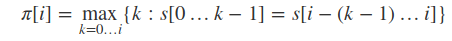
\includegraphics[width=\linewidth/2]{proper_prefixes.png}
        
        For example, for the pattern \texttt{abcdeabc}, the prefix function array will be [0, 0, 0, 0, 0, 1, 2, 3]
        
        Most of the string matching algorithms are using prefix function to minimize the cost of the algorithm.
        
        \begin{minted}[frame=lines,linenos,fontsize=\footnotesize]{c++}
vector <int> prefix_array;
void calculatePrefixArray(string pattern){
    int len = 0; // length of the current proper prefix
    int i = 1;   // pointer that traverse on pattern 
    prefix_array.resize(pattern.size());
    prefix_array[0] = 0;
    
    while(i < pattern.size()){
        if(pattern[i] == pattern[len]){
            prefix_array[i] = ++len;
            i++;
        }else{
            if(len != 0){ // if i had a proper prefix before
                len = prefix_array[len-1];
            }else{
                prefix_array[i] = 0;
                i++;
            }
        }
    }
}
        \end{minted}
        
        \subsection{KMP}
        KMP string matching algorithm is performed very similarly to the naive approach. In the case of a mismatch while checking a substring for whether it is equal to the pattern or not, we do not start over. Instead, we start from the head of the proper prefix we have matched so far if there is any. Because if we have a proper prefix, means that we have a suffix that is equal to the prefix. The pattern we am looking for might be starting with this very suffix we just found. 
        
        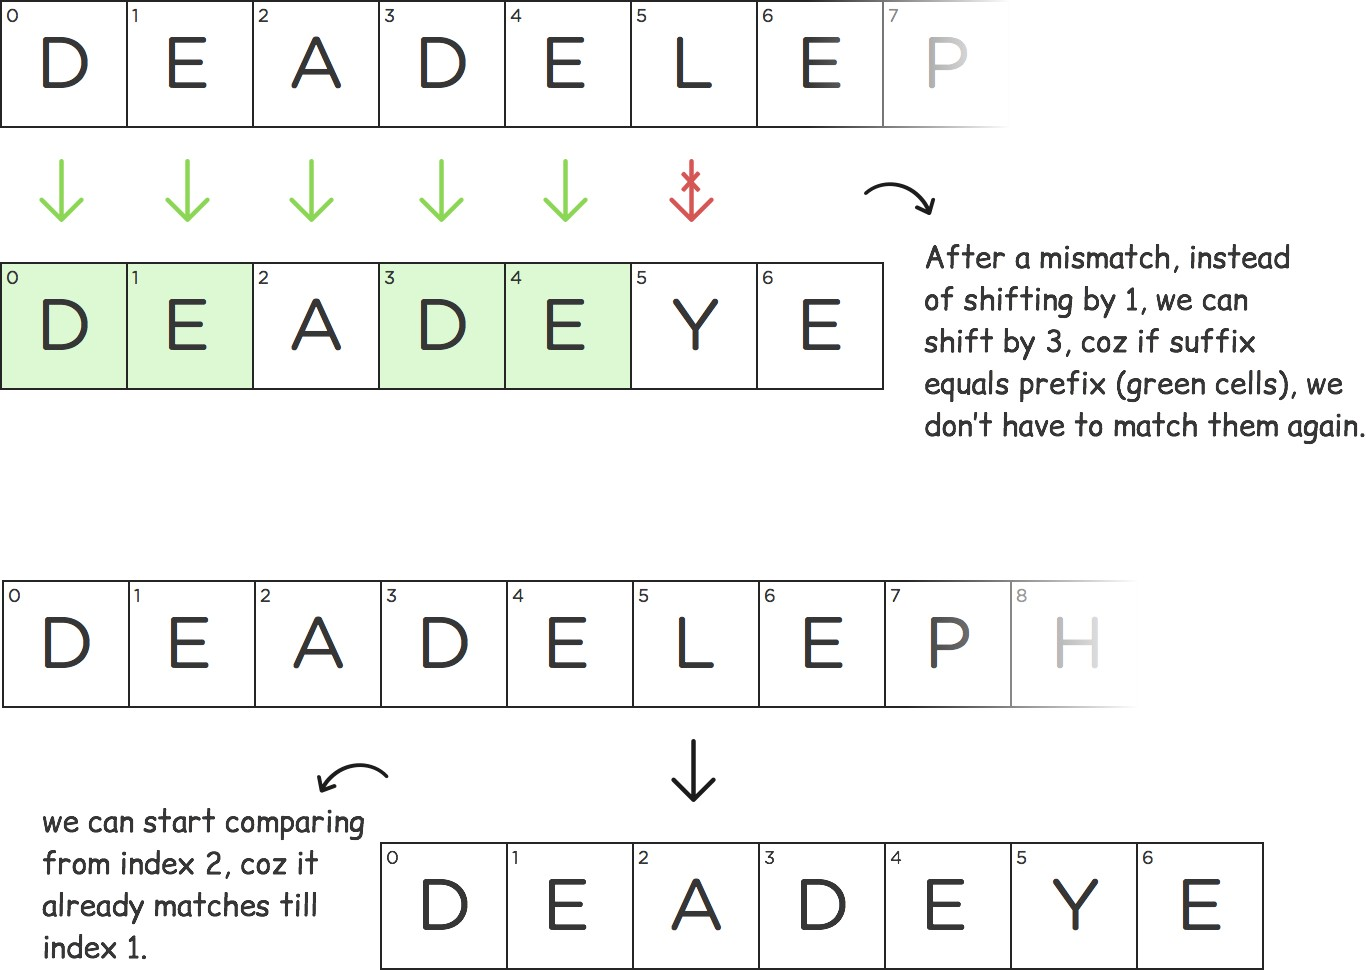
\includegraphics[width=\linewidth/1]{kmp.jpeg}
        
        \newpage
        
        \begin{minted}[frame=lines,linenos,fontsize=\footnotesize]{c++}
bool KMP(string text, string pattern){
    calculatePrefixArray(pattern);
    int i = 0; // pointer to traverse on text
    int j = 0; // pointer to traverse on pattern

    while(i < text.size()){
        if(j==pattern.size()) return true;

        if(text[i] == pattern[j]){
            i++;
            j++;
        }else{
            if(j != 0){
                /*
                if i had a matching sequence lately
                do not go to the beginning
                go to the beginning of the proper prefix
                and do not increment i
                */ 
                j = prefix_array[j-1];
            }else{
                // increment i
                i++;
            }
        }
    }

    return j == pattern.size();
}
        \end{minted}
        
        The time complexity for KMP is \texttt{O(m+n)} and memory complexity is \texttt{O(n)}.
        
        \subsection{String Matching Automata}
        In string matching automata, we precalculate a pattern and build a 2D array that represents a Finite Automata. We will search for the pattern in the text according to this array. It will tell us which state to go next, according to the current state we are in. Calculation of the state table is the tricky part of this algorithm. This algorithm is useful while dealing with the relatively small sized pattern texts and alphabets, and large size of input texts.
        
        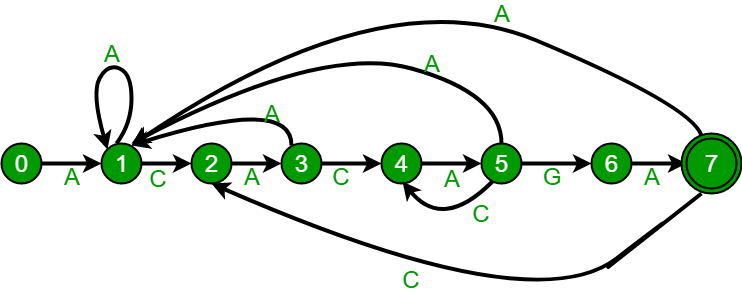
\includegraphics[width=\linewidth/2]{autometa1.png}
        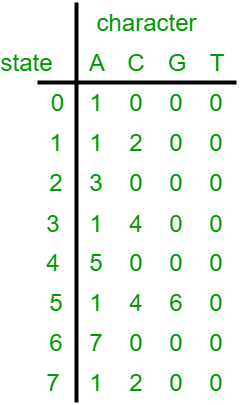
\includegraphics[width=\linewidth/5]{autometa2.png}
        
        The size of the state array will be \texttt{size of the alphabet * (size of the pattern + 1)}. We will be on \texttt{state(0)} at the beginning.
        
        Let's say we are at the state \texttt{t} and checking for the letter \texttt{l} of the alphabet. Now, what we should do is consider the string \texttt{pat[0...t-1] + l}. Let's call this new string \texttt{newPattern}. Our next state will be the length of the longest proper prefix of the string \texttt{pat + '#' + newPattern}. The character '#' is placed in the middle of two strings to distinguish them (make sure '#' is not in the given alphabet or choose one outside from the alphabet).
        
        \begin{minted}[frame=lines,linenos,fontsize=\footnotesize]{c++}
int state_table[N+1][M];
// N=length of the input, M=size of the alphabet
void create_state_table(string pattern, string alphabet){
    string pat = "";
    for(int i=0; i<pattern.size()+1; i++){
        for(int j=0; j<alphabet.size(); j++){
            string tmp = pat;
            pat += alphabet[j];
            //cerr << pat << endl;
            int new_state=0, pattern_ptr=0;

            prefix_array.clear();
            calculatePrefixArray(pattern + '#' + pat);

            new_state = prefix_array[pattern.size() + i + 1];
            
            state_table[i][j] = new_state;
            pat = tmp;
        }
        if(i < pattern.size()) pat += pattern[i];
    }
}
        \end{minted}
        
        Time complexity for building the state table is \texttt{O(n*m)} (n is the size of the pattern and m is the size of the alphabet).
        
        \newpage
        
        While searching for the pattern in the text, we simply follow our state table. If we reach the last state, it means we have found the pattern.
        
        \begin{minted}[frame=lines,linenos,fontsize=\footnotesize]{c++}
bool finite_automata(string pattern, string text, string alphabet){
    create_state_table(pattern, alphabet);
    int current_state = 0;
    int last_state = pattern.size();
    
    for(int i=0; i<text.size(); i++){
        current_state = state_table[current_state][s[i]];
        if(current_state == last_state) return true;
    }
    return false;
}
}
        \end{minted}
        
        \subsection{Rabin-Karp Algorithm}
        This algorithm is the only string matching algorithm among the ones we are discussing that does not use prefix function.
        
        By the definition of hash, a string's hash value can be considered as unique. So if two hash values of two strings are equal, these two strings are same. By using this, we can tell if two substrings are matching or not. There is very very small probabilty(Birthday Paradox\cite{birth}) of that different strings have same hash value, but we can assume it is impossible. 
        
        \begin{minted}[frame=lines,linenos,fontsize=\footnotesize]{c++}
bool is_same(string& a, string& b){
    return hash(a) == hash(b);
}
        \end{minted}
        How can we use this in string matching? Let's say we are looking for pattern $p$ in text $t$. Length of these strings are $n$ and $m$, respectively. We will traverse in each substring of $p$ of length $n$ in $O(m)$ and check whether they are equal or not. In naive solution, this goes to complexity of $O(n*m)$. But thanks to the properties of hashing we discussed above, checking two string complexity is reduced to $O(1)$, so total complexity is with hashing average $O(m+n)$ but worst case is $O(n*m)$\cite{rabin}.
        

        
        If we know hash(str[i..j]) we can easily calculate hash(str[i + 1..j+ 1]) with using properties of rolling hash.
        
        remember rolling hash: $hash(s) = (s[0] * p^{(k)}+ s[1] * p ^ {(k-1)} + ... + s[k] * p^0) \pmod{b}$
        
        $hash(str[i....i+k]) = (s[i] * p^{(k)}+ s[i+1] * p ^ {(k-1)} + ... + s[i + k] * p^0) \pmod{b}$\newline
        $hash(str[i+1....i+k+1]) = (s[i+1] * p^{(k)}+ s[i+1] * p ^ {(k-1)} + ... + s[i + k + 1] * p^0) \pmod{b}$
        
        We can see that: \newline$hash(str[i+1....i+k+1]) = (hash(str[i....i+k]) - (s[i+1] * p^{(k)}))*p + s[i + k + 1] * p^0 \pmod{b}$
        
        \begin{minted}[frame=lines,linenos,fontsize=\footnotesize]{c++}
bool rabin_karp(string& text, string& pattern){

    int m = text.size();
    int n = pattern.size();
    int p = 271; //same p using in hash_func
    long long int mod = 1e9 + 7 //same mod using in hash_func
    long long int hash_substring, hash_pattern;
    hash_substring = hash_func(string(text.begin(), text.begin() + n));
    hash_pattern = hash_func(pattern);

    if(hash_substring == hash_pattern)
        return true;

    for(int i = n; i<m; i++){
        hash_substring = 
            ((hash_substring - (text[i - n] * p^(n-1)))*p + text[i] * p^0) % mod;
        if(hash_substring == hash_pattern)
            return true;
    }

    return false;
}
    \end{minted}
        
        \subsection{Suffix Array}
        Suffix Array is a very efficient data structure that is being widely used in compression, bioinformatics and in areas that string manipulation is used. 
        
        The problem we will be interested in is pattern finding.
        
        Suffix Array is a sorted array consisting of all suffixes of a string.
        
        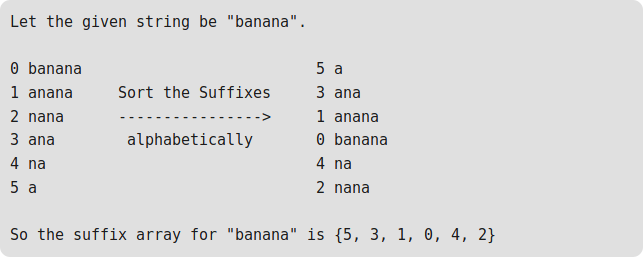
\includegraphics[width=\linewidth/2]{suffix_array1.png}
        
        
        \subsubsection{Naive Approach}
        
        Naive Approach has a complexity of $O(n^2 * log(n))$ and n is the length of the string. In naive approach, we simply traverse through all suffixes of the string and store them in an array. While sorting this array, we get $O(n^2 * log(n))$ since comparing two strings is $O(n)$.
        
        \subsubsection{$O(n * log(n) * log(n))$ Algorithm}
        
        One can observe that the suffixes we are trying to sort belong to the same string. By using this fact, we will first sort suffixes by their first character, and then we will sort suffixes of length two, and then of length four, and the length of the suffixes we will compare will grow exponentially. We will be performing sorting operation in $O(log(n))$ step, therefore we have a complexity of $O(n * log(n) * log(n))$.
        
\begin{minted}[frame=lines,linenos,fontsize=\footnotesize]{c++}
#define MAXN 65536
#define MAXLG 17
char A[MAXN];
struct entry
{
    int nr[2];
    int p;
} L[MAXN];
int P[MAXLG][MAXN];
int N,i;
int stp, cnt;
int cmp(struct entry a, struct entry b){
    return a.nr[0]==b.nr[0] ?(a.nr[1]<b.nr[1] ?1: 0): (a.nr[0]<b.nr[0] ?1: 0);
}
int main()
{
    gets(A);
    for(N=strlen(A), i = 0; i < N; i++)
    P[0][i] = A[i] - 'a';
    for(stp=1, cnt = 1; cnt < N; stp++, cnt *= 2)
    {
        for(i=0; i < N; i++){
            L[i].nr[0]=P[stp- 1][i];
            L[i].nr[1]=i +cnt <N? P[stp -1][i+ cnt]:-1;
            L[i].p= i;
        }
        sort(L, L+N, cmp);
        for(i=0; i < N; i++)
            P[stp][L[i].p] =i> 0 && L[i].nr[0]==L[i-1].nr[0] && L[i].nr[1] == L[i- 1].nr[1] ? P[stp][L[i-1].p] : i;
    }
    return 0;
}

\end{minted}
        \newpage
        \subsubsection{Pattern Finding}
        
        Since our suffix array is sorted, we can perform search operation efficiently by using binary search.
        
\begin{minted}[frame=lines,linenos,fontsize=\footnotesize]{c++}
    // A suffix array based search function to search a given pattern 
    // 'pat' in given text 'txt' using suffix array suffArr[] 
void search(char *pat, char *txt, int *suffArr, int n) 
{ 
    int m = strlen(pat);  // get length of pattern, needed for strncmp() 
  
    // Do simple binary search for the pat in txt using the 
    // built suffix array 
    int l = 0, r = n-1;  // Initilize left and right indexes 
    while (l <= r) 
    { 
        // See if 'pat' is prefix of middle suffix in suffix array 
        int mid = l + (r - l)/2; 
        int res = strncmp(pat, txt+suffArr[mid], m); 
  
        // If match found at the middle, print it and return 
        if (res == 0) 
        { 
            cout << "Pattern found at index " << suffArr[mid]; 
            return; 
        } 
  
        // Move to left half if pattern is alphabtically less than 
        // the mid suffix 
        if (res < 0) r = mid - 1; 
  
        // Otherwise move to right half 
        else l = mid + 1; 
    } 
  
    // We reach here if return statement in loop is not executed 
    cout << "Pattern not found"; 
} 
\end{minted}

    Note that in the above implementation, \texttt{suffArr[i]} corresponds to $i'th$ suffix of a string. For example let that string be $"banana"$ and $i$ be one.
    
    \texttt{suffArr[i] = 3}
    \texttt{string[3..n] = "ana"}
    
    \newpage
    
        \subsection{LCP Array}
        LCP means longest common prefix. \texttt{LCP[i]} holds the length of the longest common prefix of \texttt{suffArr[i]} and \texttt{suffArr[i+1]}.
        
        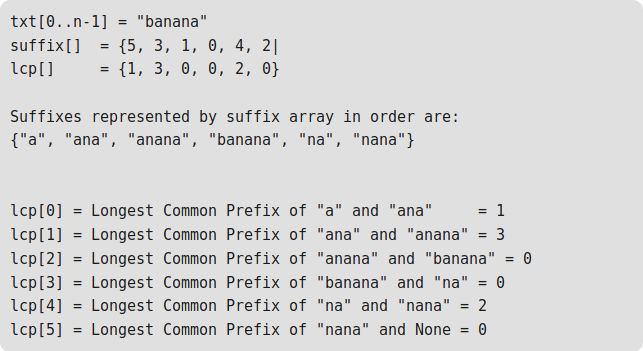
\includegraphics[width=\linewidth/1]{lcp.png}
        
        There are many ways to construct a LCP Array but we are going to discuss the one that uses precalculated suffix array (Kasai's Algorithm).
        
\begin{minted}[frame=lines,linenos,fontsize=\footnotesize]{c++}
int lcp(int x, int y){
    // lcp's of substring s[x..n] and s[y..n]
    int res = 0;
    for(int i=logn; i>=0; i--){
        if(P[i][x] == P[i][y]){
            res += pow(2, i);
            x += pow(2, i);
            y += pow(2, i);
        }
        // move to the next characters
    }
    return res;
}
\end{minted}

    The algorithm above has a complexity of $O(log(n))$ and should be called for each suffix so its total complexity is $O(n*log(n))$.
        
       \newpage
       \section{References}
        
        \begin{thebibliography}{0}
            
            \bibitem{sa}
            https://www.geeksforgeeks.org/suffix-array-set-2-a-nlognlogn-algorithm/
            \bibitem{pf}
            https://cp-algorithms.com/string/prefix-function.html
            \bibitem{gfg}
            https://www.geeksforgeeks.org/suffix-array-set-2-a-nlognlogn-algorithm/
            \bibitem{cp}
            https://cp-algorithms.com/string/string-hashing.html
            \bibitem{kasai}
            https://www.geeksforgeeks.org/kasais-algorithm-for-construction-of-lcp-array-from-suffix-array/
            \bibitem{fa}
            https://www.geeksforgeeks.org/finite-automata-algorithm-for-pattern-searching/
            \bibitem{rk}
            https://cp-algorithms.com/string/rabin-karp.html
            \bibitem{birth}
            https://en.wikipedia.org/wiki/Birthday\_paradox
            \bibitem{rabin}
            https://en.wikipedia.org/wiki/Rabin-Karp\_algorithm
        \end{thebibliography}
    
    \end{document}